\section{Reproducibility and Evidence Traceability}\label{sec:repro}

\subsection{Replication Package}
The implementation, development records, raw result files and manuscript sources are in the project repository on branch \code{research/v8-linux-validation}. The placebo, frozen-threshold and profile-fix results come from branch \code{research/v8-mac-hardening} (commits \code{8e28f601}, \code{b9b8a86c}). Table~\ref{tab:artifacts} maps each result to its raw source and the script that derives it. A reproducing group needs Python~3.11 or later with NumPy, SciPy and Matplotlib. The statistical recomputation takes about one minute and executes no program under test. Re-collecting evidence additionally requires the V7-B engine and an operating-system sandbox (\code{sandbox-exec} on macOS, \code{bwrap} on Linux).

\begin{table*}[!t]
\caption{Artifact provenance. Class: R = raw machine-readable output; D = derived by a script from R; M = manuscript calculation; C = conceptual. Raw: raw output present in the repository. Tree: state of the code when the output was produced (clean, dirty, or unrecorded). Re-run: whether an independent group can regenerate the result from the repository (Analysis = from saved records without executing programs; Collect = requires re-executing programs). ``mac'' = branch \code{research/v8-mac-hardening}.}
\label{tab:artifacts}
\centering
\scriptsize
\setlength{\tabcolsep}{2.4pt}
\renewcommand{\arraystretch}{1.08}
\begin{tabular}{|L{2.6cm}|L{4.4cm}|c|L{1.0cm}|L{1.25cm}|L{1.45cm}|L{3.3cm}|}
\hline
Result & Source & Class & Raw & Tree & Re-run & Known gap \\
\hline
Corpus and labels & \bcode{datasets\/v8\/dev\_records.jsonl} (312 records) & R & Records only & Unrecorded & Analysis; Collect needs V7-B & Per-run logs (\bcode{results\/repro\/v8\_dev\_20261118\_195446}) absent \\
Rule and model risks, contrasts & \bcode{scripts\/stats\_recompute.py} $\to$ \bcode{audit\/stats\_summary.json} & D & Yes & Code at \code{07ecd5b7} & Analysis, about 1 min & -- \\
Seeds, B6 contrast & \bcode{results\/v8\_dev\_eval\_20261119\_*\_linux\_\{soft,strict\}} & R & Yes & Unrecorded & Analysis & Run metadata lack a commit \\
Placebo, frozen thresholds, profile fix & mac: \bcode{results\/v8\_mac\_reanalysis\_20261118\_*} & R & Yes & Commit \code{b9b8a86c} & Analysis & Fix not merged into the evaluated branch \\
\ers{} matrix & \bcode{results\/v8\/linux\/perturb\/posthoc\_matrix.json}; mac \bcode{results\/v8\_mac\_perturb\/} & R & Yes & Linux: clean flag, commit unrecorded & Analysis & -- \\
Real-execution analogue & \bcode{results\/v8\_mac\_perturb\/realexec\_matrix.json} (720 rows) & D & Matrix only & Dirty at \code{01fdaf09} & Collect & Run directories absent; uncommitted changes listed in manifest \\
Security, macOS & \bcode{audit\/security\_rerun\_darwin.json}; mac \bcode{results\/v8\_mac\_security\/} & R & Yes & \code{07ecd5b7} & Collect, about 9\,s & macOS only \\
Security, Linux & \bcode{results\/v8\/linux\/expanded\_security\_suite\_results.json} & R & Yes & Unrecorded & Collect & No host, sandbox or time metadata \\
Five-dataset audit & Generator code and manifests; \bcode{scripts\/verify\_five\_dataset.py} & D & Yes & Code at \code{07ecd5b7} & Static & -- \\
Cross-platform status & Saved outputs on both branches & M & Yes & As above & Static & -- \\
Test suite & \code{tests/v8} & R & Summary only & \code{07ecd5b7} & Collect, about 85\,s & Linux run report-only \\
Conceptual figures & \bcode{scripts\/make\_figures.py} & C & -- & -- & Static & -- \\
\hline
\end{tabular}
\end{table*}

\paragraph*{What is and is not reproducible} Reproducibility in this study has three levels.
\begin{enumerate}
\item \emph{Analysis from saved records.} Every statistic, the post-hoc \ers{} matrix, the five-dataset audit and every figure can be regenerated from files in the repository without executing any program under test. Cross-platform agreement to $10^{-9}$ shows that this level holds.
\item \emph{Re-executable collection.} The macOS security suite and the test suite can be re-executed from the repository on macOS. Re-execution yields new observations, not a replay of the reported ones.
\item \emph{Not reproducible from the repository.} The per-run logs behind the 312 development records, the run directories of the real-execution analogue, and the host metadata of the Linux security run are absent. The development records are therefore the earliest verifiable artifact, and the real-execution analogue was produced from code with uncommitted changes. Neither can be independently re-derived.
\end{enumerate}

\subsection{Claim Register and Traceability}
Every numerical statement in the paper is listed in a claim register with its section, value, raw source, derivation, branch or commit, verification mode and limitation. The register is distributed with the manuscript (\bcode{FINAL\_CLAIM\_EVIDENCE\_REGISTER.md}, \bcode{NUMERICAL\_CLAIM\_AUDIT.md}). Fig.~\ref{fig:trace} shows three example chains. Values found only in report text are listed as excluded: calibration slopes near 1, a strict-policy coverage of 47 pairs, per-seed $p$-values that disagree with raw output, container isolation through a runtime the code never invokes, and a 608-test Linux run. No experiment, benchmark run, validation run or statistical pipeline was re-executed for this revision. Tables and figures were re-derived from existing outputs only.

\begin{figure*}[!t]
\centering
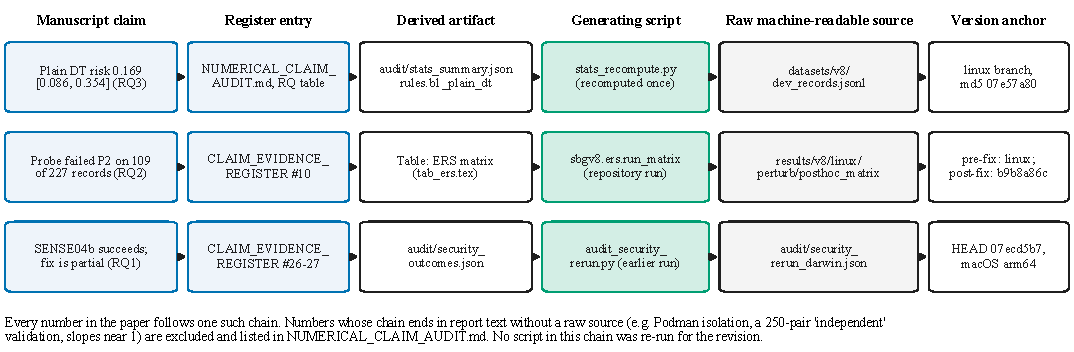
\includegraphics[width=\textwidth]{figures/fig_traceability.pdf}
\caption{Evidence-to-claim traceability: three example chains from a manuscript claim through its register entry, derived artifact and generating script to the raw machine-readable source and its version anchor.}
\label{fig:trace}
\end{figure*}

\subsection{Artifact Audit}
Before writing, we audited the project's machine-readable records against its internal reports. Three findings affect what can be claimed.
\begin{enumerate}
\item The five-dataset artifact does not meet the evidential standard (Section~\ref{sec:res-rq5}). It is classified invalid as external-validation evidence (label-derived outcomes, stub predictor, no executed benchmark, zero human verdicts) and is excluded entirely.
\item Some report figures have no raw support; they are not used.
\item The profile fix exists on a sibling branch. We report the evaluated branch's numbers and the effect of the fix separately, and merging the fix is required before any further study.
\end{enumerate}

\subsection{Adjudication Protocol and Prediction Lock}
The adjudication protocol is implemented and tested on synthetic fixtures but has not been executed.
\begin{itemize}
\item \emph{Independence.} Two adjudicators examine each change independently, within a boundary $\obs$ and budget $\budget$ that are frozen before the first decision.
\item \emph{Blinding.} The case schema has no field for model scores, \ers{} outputs or verdicts, and any such key raises an error.
\item \emph{Disagreements.} A disagreement goes to a third, distinct adjudicator whose decision is final. Without one, the case stays unresolved and enters the estimand through the variants of Section~\ref{sec:problem}.
\item \emph{Agreement.} Agreement is reported as Cohen's $\kappa$ with the confusion matrix. Scoring may begin only if $\kappa\ge0.7$ on at least 30\% double-labelled cases.
\item \emph{Records.} Decisions go into an append-only hash-chained log, which is tamper-evident but not signed.
\item \emph{Prediction lock.} Predictions are hash-sealed before adjudication. A usable lock also requires an external timestamp and an adjudication package from which labels cannot be inferred.
\end{itemize}
